\chapter{نتيجه‌گيري و پیشنهادات}

\section{نتيجه‌گيري}
در فصول پیشین با توجه به مزیت‌های ذکر شده برای ربات چهارپا و مشخصات مطلوب مدنظر، مدل نهایی طراحی شد. با انجام اصلاحاتی روی ربات، قطعات جدید پرینت شد و مدل نهایی در عمل پیاده سازی شد. در قسمت سخت‌افزار ربات، با توجه اینکه سروموتور \lr{SG90} نیاز ما را از لحاظ سبکی و گشتاور لازم برای بلند کردن و حرکت ربات و مقرون به صرفه بودن برطرف نمود از آن استفاده شد، همچنین کم بودن پایه‌های \lr{Arduino Uno} برای استفاده از \lr{PWM} منجر به استفاده از میکروکنترلر \lr{STM32F103C8T6} شد. برای تشخیص موانع موجود به دلیل قیمت مناسب، موجود در بازار و کیفیت مطلوب ماژول \lr{ESP32-CAM} به کار برده شد. به این دلیل که وزنی به ربات اضافه نشود به جای آنکه باتری بر روی ربات قرار بگیرد و موتورها را برای حرکت دادن ربات دچار مشکل کند، از منبع ولتاژ \lr{DC} استفاده شد و همچنین 12 موتور در بعضی مواقع مانند بلند شدن ربات از زمین، جریانی زیادی را می‌کشند که ممکن است باتری نتواند آن را تامین کند.
	\begin{figure}[!h]
	\centering
	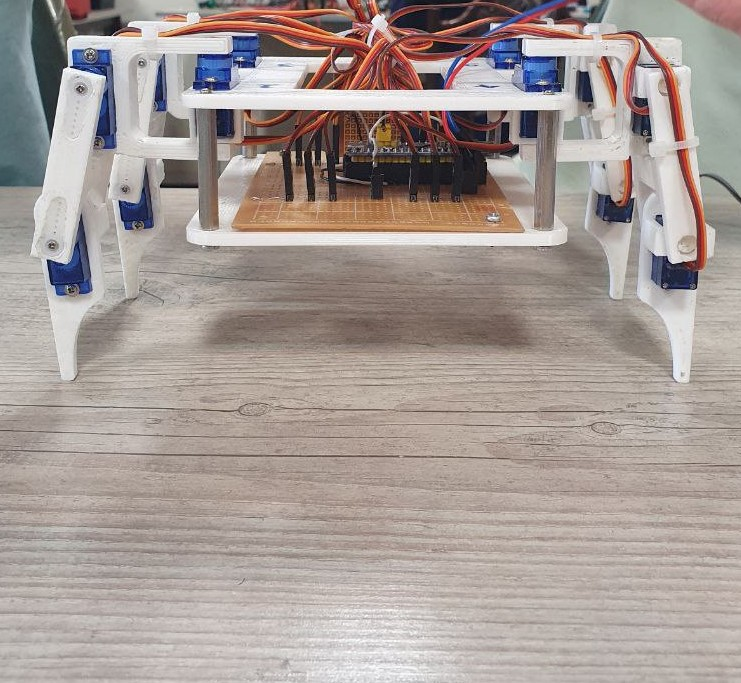
\includegraphics[width=9cm,height=9cm]{./Images/CH5/IMG_1.jpg}
	\caption{ربات نهایی}
	\end{figure}
	
\newpage
برای قسمت نرم‌افزار ربات، برای برقراری ارتباط بین میکروکنترلر و دوربین، از پروتکل \lr{UART} استفاده شد. برای حفظ تعادل و حرکت در مسیر درست، نیاز است که هر موتور دقیقاً به موقعیت مطلوب برود پس برای کنترل موقعیت و زاویه هر موتور تکنیک کنترلی \lr{PWM} به کار برده شد. برای انجام تنظیمات مورد نیاز میکروکنترلر و به جهت ساده‌تر کردن و سرعت بخشیدن به برنامه‌نویسی میکروکنترلر از نرم‌افزار \lr{CubeMX} بهره برده شد. درنهایت به دلیل رایج بودن محیط برنامه‌نویسی \lr{Keil}، برای فعال‌سازی و راه‌اندازی تایمرها و نوشتن توابع حرکتی ربات از آن استفاده شد.
	\begin{figure}[!h]
	\centering
	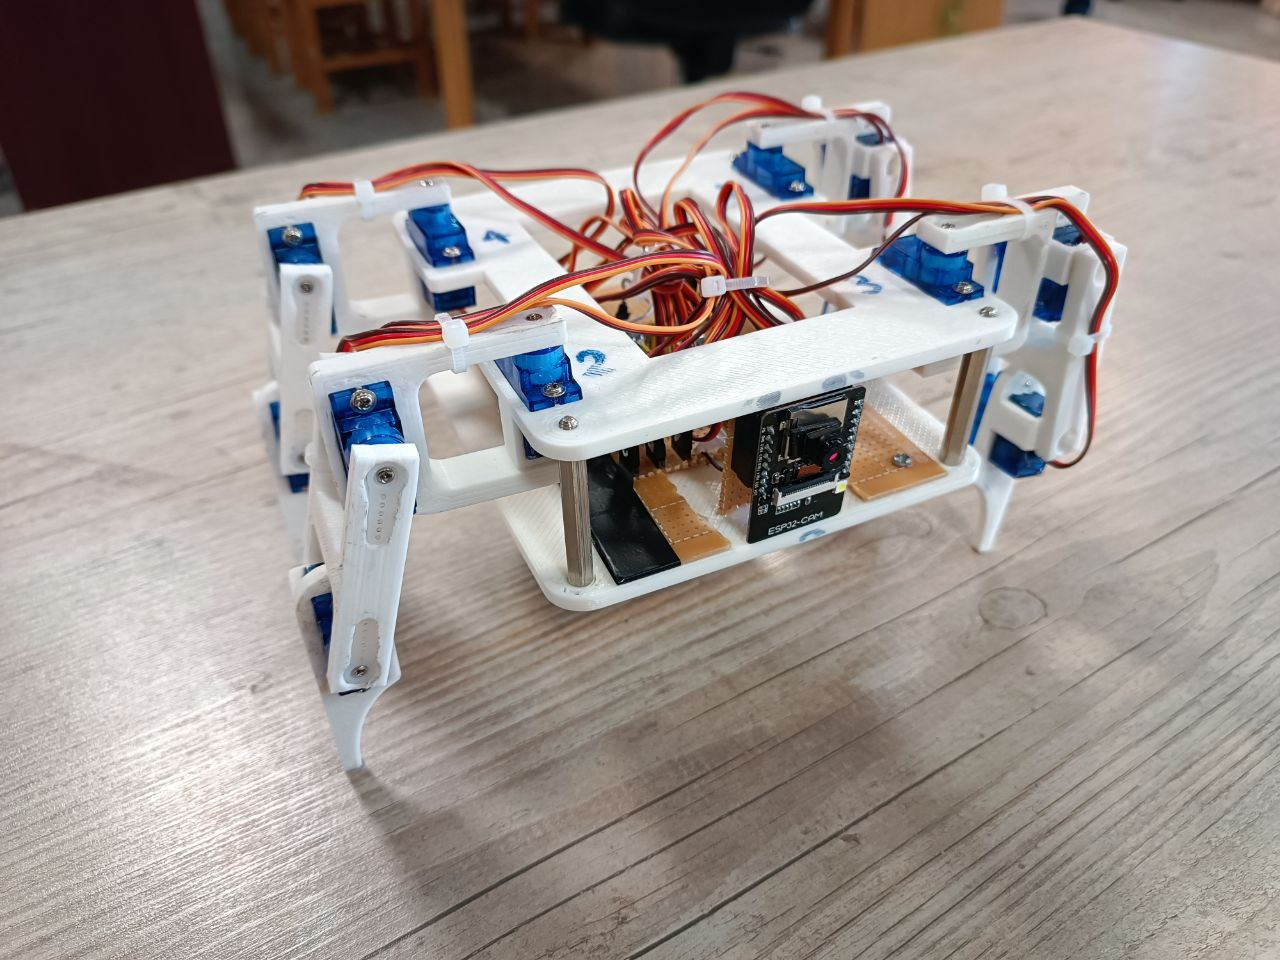
\includegraphics[width=12cm,height=9cm]{./Images/CH5/IMG_2.jpg}
	\caption{ربات نهایی}
	\end{figure}
	
\newpage
برای جابه‌جایی ربات از نقطه‌ای به نقطه دیگر از اصطکاک پاها کمک گرفته شده است و در تمام حرکت‌های ربات اعم از حرکت رو به جلو و عقب، به موتورها فرمانی داده شده است که با استفاده از اصطکاک و عکس العمل آن ربات به سمت دلخواه حرکت کند. همچنین برای بلند شدن ربات و قرارگیری در حالت اولیه، به موتورهای اول، دوم یا سوم هر پا همزمان فرمان داده می‌شود تا ربات در هنگام بلند شدن تعادل خود را نگه دارد و بدون لعزش بایستد. در شکل \ref{State0} ربات بدون هیچ دستور و ولتاژی به موتورهایش روی زمین قرار گرفته است اما با اعمال ولتاژ به موتورها و میکروکنترلر، دستور رفتن به حالت اولیه (\ref{State1}) اتفاق می‌افتد.
    \begin{figure}[!h]
	\centering
	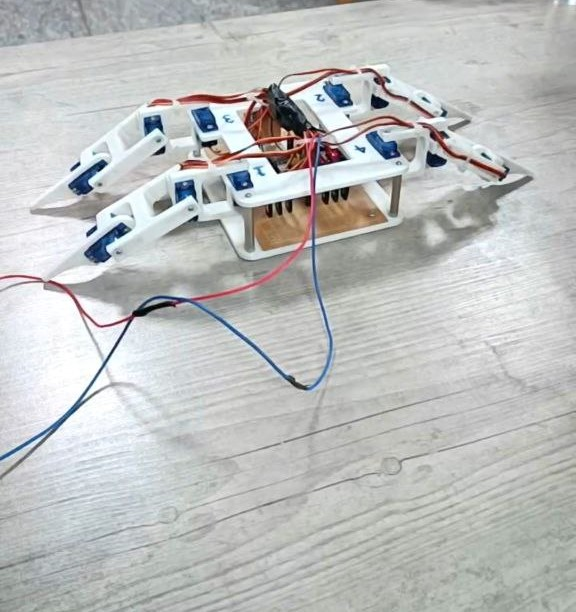
\includegraphics[width=7.5cm,height=7.5cm]{./Images/CH5/State0.jpg}
	\caption{ربات بدون هیچ فرمان}
	\label{State0}
	\end{figure}
	\begin{figure}[!h]
	\centering
	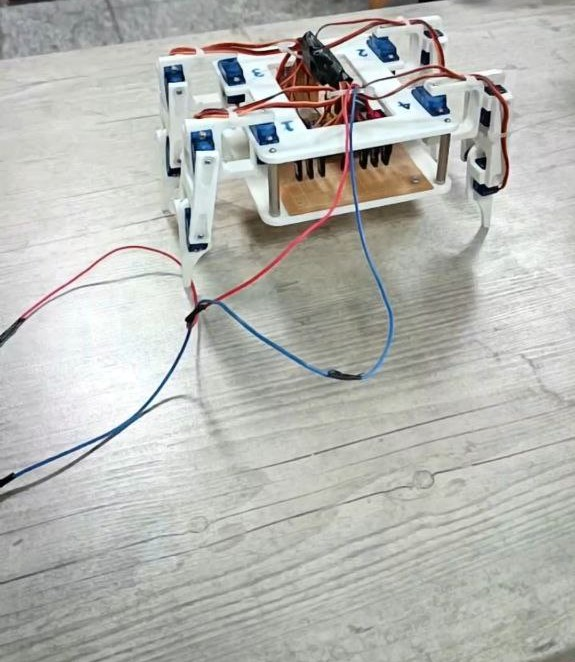
\includegraphics[width=7.5cm,height=7.5cm]{./Images/CH5/State1.jpg}
	\caption{ربات در حالت اولیه}
	\label{State1}
	\end{figure}
	
\section{پیشنهادات}
با توجه به تجربیاتی که از ساخت ربات بدست آوردیم، بهتر است از سروموتورهای قوی‌تر و بهتری استفاده شود که در حرکت دادن پاهای ربات مشکلی وجود نداشته باشد و همچنین بهتر است پای دوم کوتاه‌تر از پای سوم باشد و به شکلی ربات قرار بگیرد که در حالت اولیه ربات که ربات ایستاده است؛ بدنه از مفصل پای سوم پایینتر باشد و به زمین نزدیک باشد. مهمترین نکته هم آن است که چرخ‌دنده‌های موتورها پلاستیکی نباشد چون با کوچکترین فشاری از خارج به ربات باعث شکستن چرخ‌دنده می‌شود.

اگر از سروموتور قوی‌تری استفاده شود، می‌توان بدنه را کمی سبکتر ساخت و دیگر نیازی به منبع ولتاژ ثابت نباشد و به جای آن از باتری استفاده گردد که جابه‌جایی ربات آسان‌تر انجام شود چون وجود دو سیم منبع ولتاژ می‌تواند مانع انجام درست جرکت‌ها شود (فقط به این توجه شود که باتری توان جریان‌کشی زیاد موتورها را داشته باشد).

به جای حرکت به کمک اصطکاک بهتر است که طراحی به شکلی صورت گیرد که ربات قادر به گام‌برداری باشد به صورتی که اگر یک پا از زمین جدا شود و به سمتی حرکت کند ربات تعادل داشته باشد و واژگون نشود. به این ترتیب ربات وابستگی به جنس محیط برای داشتن اصطکاک مطلوب ندارد.